% The MIT License (MIT)
% =====================

% **Copyright (c) 2018 Anish Athalye (me@anishathalye.com)**

% Permission is hereby granted, free of charge, to any person obtaining a copy of
% this software and associated documentation files (the "Software"), to deal in
% the Software without restriction, including without limitation the rights to
% use, copy, modify, merge, publish, distribute, sublicense, and/or sell copies
% of the Software, and to permit persons to whom the Software is furnished to do
% so, subject to the following conditions:

% The above copyright notice and this permission notice shall be included in all
% copies or substantial portions of the Software.

% THE SOFTWARE IS PROVIDED "AS IS", WITHOUT WARRANTY OF ANY KIND, EXPRESS OR
% IMPLIED, INCLUDING BUT NOT LIMITED TO THE WARRANTIES OF MERCHANTABILITY,
% FITNESS FOR A PARTICULAR PURPOSE AND NONINFRINGEMENT. IN NO EVENT SHALL THE
% AUTHORS OR COPYRIGHT HOLDERS BE LIABLE FOR ANY CLAIM, DAMAGES OR OTHER
% LIABILITY, WHETHER IN AN ACTION OF CONTRACT, TORT OR OTHERWISE, ARISING FROM,
% OUT OF OR IN CONNECTION WITH THE SOFTWARE OR THE USE OR OTHER DEALINGS IN THE
% SOFTWARE.


% Gemini theme
% https://github.com/anishathalye/gemini

\documentclass[final]{beamer}

% ====================
% Packages
% ====================

\usepackage[T1]{fontenc}
\usepackage{lmodern}
\usepackage[size=custom,width=130 ,height=100,scale=1.0]{beamerposter}
\usetheme{gemini}
\usecolortheme{gemini}
\usepackage{graphicx}
\usepackage{booktabs}
\usepackage{tikz}
\usepackage{pgfplots}
\usepackage{tcolorbox}
\usepackage{geometry}

% ====================
% Lengths
% ====================

% If you have N columns, choose \sepwidth and \colwidth such that
% (N+1)*\sepwidth + N*\colwidth = \paperwidth
\newlength{\sepwidth}
\newlength{\colwidth}
\setlength{\sepwidth}{0.025\paperwidth}
\setlength{\colwidth}{0.3\paperwidth}

\newcommand{\separatorcolumn}{\begin{column}{\sepwidth}\end{column}}

% ====================
% Title
% ====================

\title{Developing a QIIME 2 Plugin - a Simple Annotation for Robust Tools}

\author{Christopher R. Keefe \and Evan Bolyen \and Matthew Ryan Dillon \and J. Gregory Caporaso}

\institute[shortinst]{The Center for Applied Microbiome Science, Pathogen and Microbiome Institute, Northern Arizona University}

% ====================
% Body
% ====================

\begin{document}

\begin{frame}[t]
\begin{columns}[t]
\separatorcolumn

\begin{column}{\colwidth}

  \begin{block}{Objective and Introduction}

    \textbf{Introduction:}
    Developers of computational methods for microbiome science can greatly increase
    the robustness and accessibility of their software, improve distribution and citation,
    and facilitate the integration of their methods with new and existing analytical
    pipelines by taking advantage of existing QIIME 2 \cite{10.7287/peerj.preprints.27295v1}
    infrastructure. Doing so can be as simple as wrapping a script in a Python 3
    package, then annotating with information about the commands it makes available, the
    parameters they expose, and the types of data they input and output. Additional
    resources exist in the QIIME 2 ecosystem for developers who wish to disseminate and
    support their methods, or collaborate with other developers.
    \hfill\break

    \begin{figure}[tph!]
    {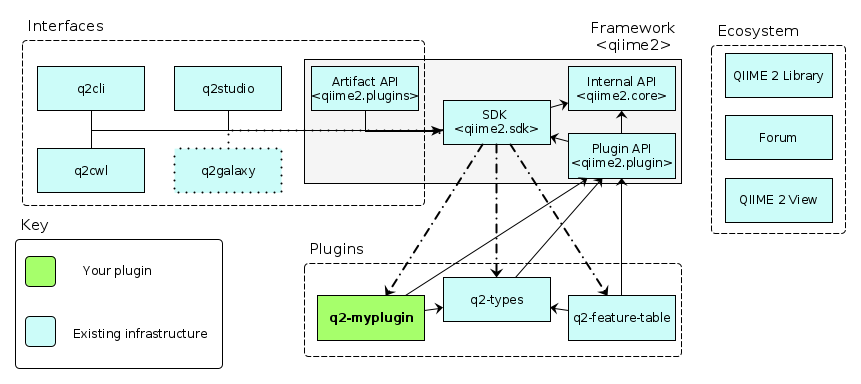
\includegraphics[height=16cm]{assets/infrastructure_diagram_bicolor}}
    \caption{\,QIIME 2 plugins reduce development overhead by utilizing existing infrastructure (blue).}
    \label{fig:infrastructure}
    \end{figure}

    \textbf{QIIME 2 provides:}
    \begin{itemize}
      \item \textbf{Interfaces:} Familiar user interfaces for a diverse
      user base (e.g. CLI, API, GUI, CWL)
      \item \textbf{Community:} A vibrant user base, free forum infrastructure for
      plugin support
      \item \textbf{Visibility:} Centralized plugin dissemination through the QIIME 2
      Library
      \item \textbf{Provenance:} Integrated and automatic tracking of data provenance
      ensures reproducibility.
      \item \textbf{Citation support:} Built-in citation tracking supports attribution.
      \item \textbf{Low-level infrastructure:} Facilitates data I/O, communication
      between disparate methods in an analytical pipeline, and cross-platform compatability
      \item \textbf{Semantic typing:} A rich and extensible type system prevents user
      error, supports backwards compatability and collaboration
      \item \textbf{Sharing:} QIIME 2 View allows convenient sharing of QIIME 2 Results
    \end{itemize}
  \end{block}


  \begin{block}{Develop a method or algorithm}
  In order to develop a QIIME 2 plugin, you must first have code you would
  like to run in QIIME 2. Your method may be written Python 3, or in any
  language accessible to Python 3 with a sub-process call: popular plugins wrap
  code written in R and C, and many other options exist.\\
  \hfill\break
  Example: the q2-alignment plugin wraps the MAFFT application by importing \code{subprocess}, generating I/O filepaths, building a command for the OS, and using that command to run MAFFT.\\
      \begin{tcolorbox}
    [width=\textwidth, colframe=blue]
      {
{\texttt{\textcolor{codeblack}{
import subprocess\\
from q2\_types.feature\_data import DNAFASTAFormat, AlignedDNAFASTAFormat\\
\begin{tabbing}
def \=maff\=t(se\=quences: DNAFASTAFormat,\\
\>\>n\_threads: int = 1,\\
\>\>parttree: bool = False) -> AlignedDNAFASTAFormat:\\
\>unaligned\_filepath = str(sequences.path)\\
\>result = AlignedDNAFASTAFormat()\\
\>aligned\_filepath = str(result.path)\\
\\
\>cmd = ["\=mafft", "--preservecase", "--inputorder",\\
\>\>\>"--thread", str(n\_threads), unaligned\_filepath]\\
\\
\>with open(aligned\_filepath, 'w') as output\_f:\\
\>\>subprocess.run(cmd, stdout=output\_f, check=True)
\end{tabbing}}}}
      }
    \end{tcolorbox}
  \end{block}

  \begin{block}{Annotate your method}
    Plugin annotation allows the QIIME 2 framework to recognize and communicate with plugins.
    Annotation is simple (see Figure ~\ref{fig:registrationDiagram}), and allows plugin documentation
    to be generated in any interface. Citation information registered in plugins
    is automatically captured in Result provenance.

    To annotate a plugin:

    \begin{enumerate}
      \item Import any necessary dependencies from other plugins.
      \item Use \code{Plugin()} to instantiate your plugin.
      \item Use \code{register\_function()} to register \textit{each} public Action the plugin offers
      \item Use \code{register\_semantic\_types()} and \code{register\_semantic\_type\_to\_format()} to register any new semantic types or formats available in this plugin.
    \end{enumerate}
  \end{block}

\end{column}

\separatorcolumn

\begin{column}{\colwidth}

\begin{block}{Introduce new kinds of data}
  Some computational methods require the creation of novel data formats, or
  entirely new types of data. By defining these as Semantic Types in your plugin,
  you allow other QIIME 2 plugins to recognize and use your new data types effectively.
  Assigning semantic types to computed Results allows them to be interpreted by
  any other plugin. This "common language" enables the composition of analytical pipelines.

    \begin{tcolorbox}
    [width=\textwidth, colframe=blue]
    {NOTE: The creation of new Semantic Types is a great opportunity for collaboration
    with other developers in the field. Well-architected Types benefit analytical pipeline
    development, and help improve QIIME 2's "understanding" of microbiome data. Further,
    a clear understanding of the Types your method interacts with can clarify and improve the method
    development process.}
    \end{tcolorbox}
  \end{block}

  \begin{block}{Visualizations}
    \begin{figure}[tph!]
    {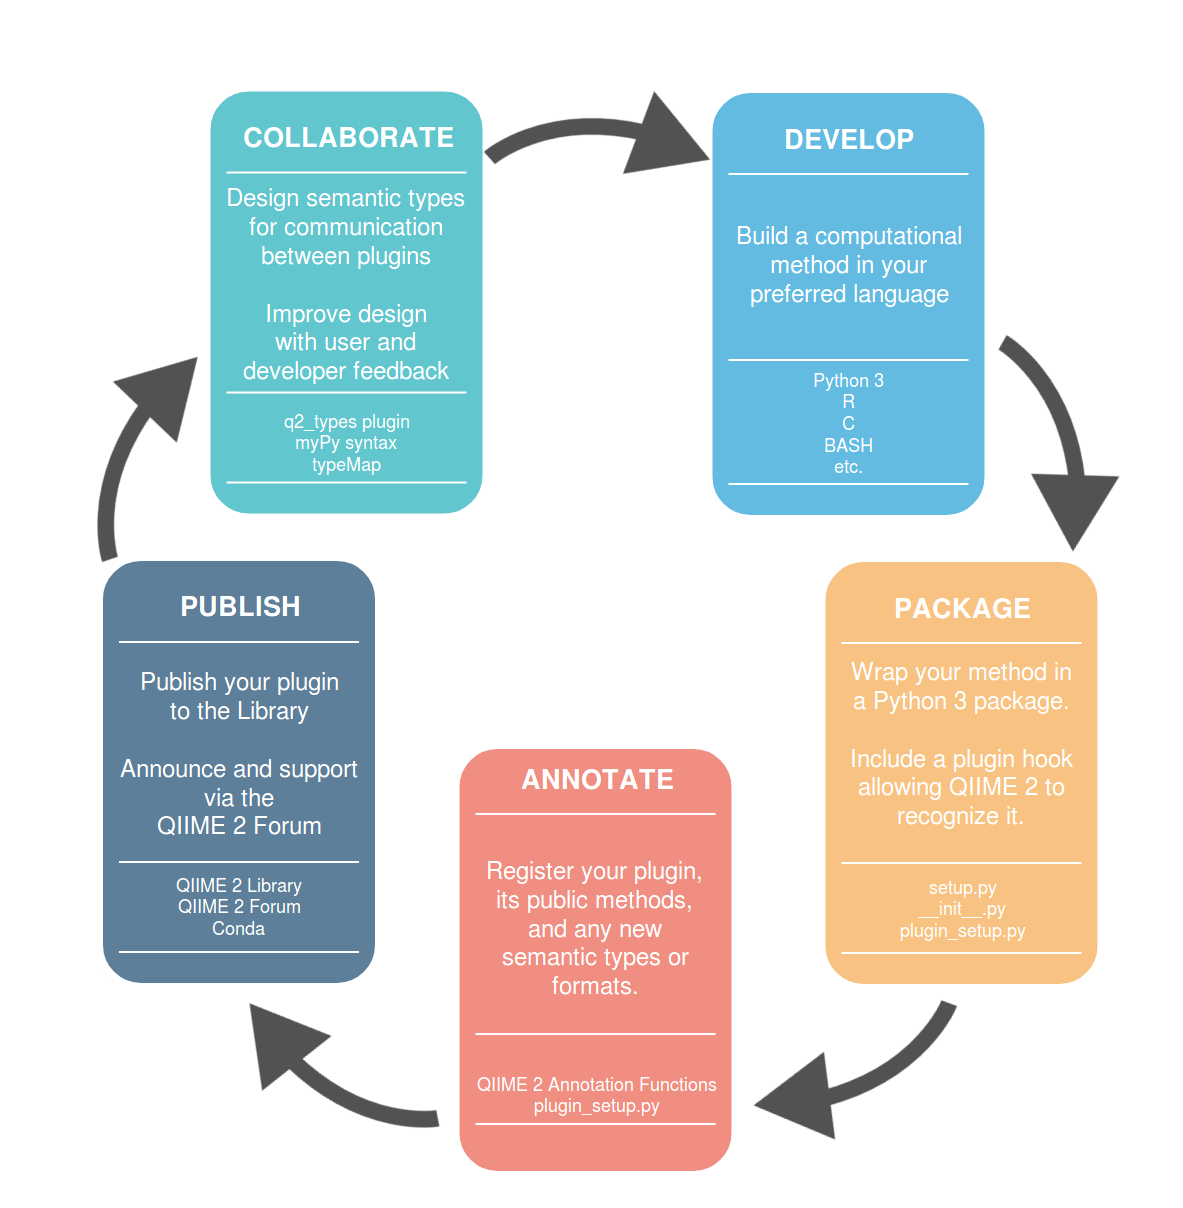
\includegraphics[height=28cm]{assets/DevelopmentProcessDiagramFlattop}}
    \caption{\,QIIME 2 plugin development cycle }
    \label{fig:processDiagram}
    \end{figure}

    \begin{figure}[tph!]
    {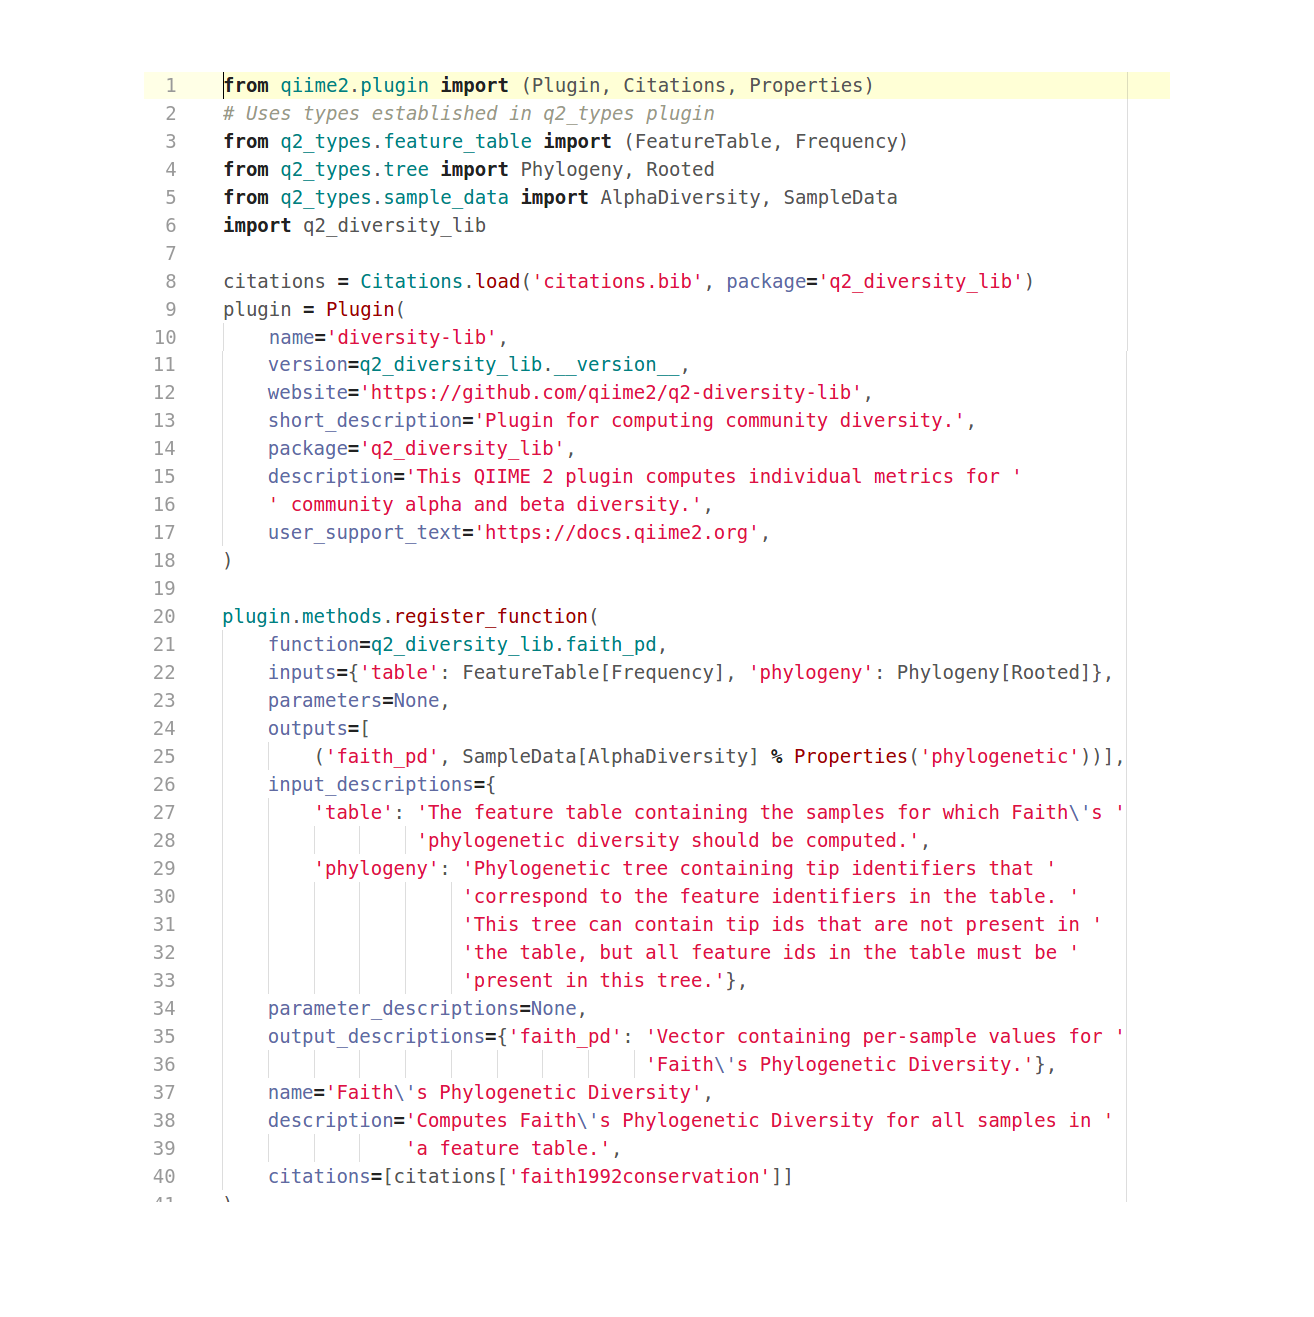
\includegraphics[width=\textwidth]{assets/registrationDiagram}}
    \caption{\,Overview of registration annotation for QIIME 2 plugins}
    \label{fig:registrationDiagram}
    \end{figure}

  \end{block}

  \begin{block}{Project Funding}
      \begin{figure}[!htb]
        \minipage{0.31\textwidth}%
          \begin{center}
            
\includegraphics[width=.35\linewidth]{assets/SponsorLogos/ABOR}
          \end{center}
        \endminipage
        \hskip 2cm
        \minipage{0.31\textwidth}
          \begin{center}
            
\includegraphics[width=.42\linewidth]{assets/SponsorLogos/APSloanFdn}
          \end{center}
        \endminipage\hfill
        \minipage{0.31\textwidth}
          \begin{center}
            
\includegraphics[width=.50\linewidth]{assets/SponsorLogos/NSF}
          \end{center}
        \endminipage\hfill
      \end{figure}
  \end{block}
\end{column}

\separatorcolumn

\begin{column}{\colwidth}

  \begin{block}{Create a Python package}

    Plugins are Python packages with metadata hooks QIIME 2 uses to facilitate
    communication between plugins. Packaging
    simplifies plugin installation, and provides access to the QIIME 2 platform.

    \begin{tcolorbox}
    [width=\textwidth, colframe=blue]
    {Python packaging may be the most challenging part of plugin creation
    for new developers, because software structure impacts package structure.
    Generally, the structure resembles Figure ~\ref{fig:packageStructure}}
    \end{tcolorbox}

    General guidelines:
    \begin{itemize}
      \item Define one or more Python 3 functions in a package
      \item Include \code{\_\_init\_\_.py} files for every subpackage of your
      plugin (a requirement of Python packages).
      \item In your \code{plugin\_setup.py}, instantiate a \code{qiime2.plugin.Plugin} object
      \item In your plugin package's \code{setup.py}, define that instance as an entry point
    \end{itemize}
  \end{block}

  \begin{figure}[tph!]
    {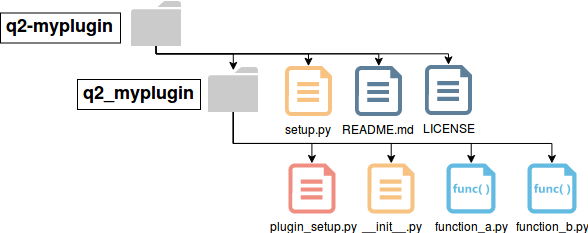
\includegraphics[height=10cm]{assets/packageStructure}}
    \caption{\,File map of a simple Python package. Note \code{plugin\_setup.py} required for QIIME 2 plugins.}
    \label{fig:packageStructure}
  \end{figure}

  \begin{block}{Publish and support}

    Completed plugins may be disseminated through the QIIME 2 Library, and announced
    in the Community Contributions category of the QIIME 2 forum. Many developers
    also use the forum as their primary platform for user support.

    Though optional, most developers distribute their plugins on Conda. This greatly
    improves dependency handling and simplifies installation.

    Plugins are often publishable as software announcements in academic journals.
    Recently-published plugins include \code{q2-perc-norm}\cite{Gibbons1006102},
    \code{q2-itsexpress}\cite{Rivers15704-1}, and \code{DEICODE}\cite{Martinoe00016-19}.

  \end{block}

  \begin{block}{Future capabilities}

    \begin{itemize}
      \item \textbf{TypeMap:} A new type map system will launch in QIIME 2 2019.4,
      giving developers powerful new tools for manipulating and constraining the types of
      data used and produced by Actions. TypeMap will allow plugins to assign
      nuanced types to their outputs programatically (e.g. based on parameterization),
      and will enhance plugins' ability to intelligently constrain allowable data inputs
      even through user-defined workflows.
      \item \textbf{\code{q2galaxy:}} A new Galaxy interface (\code{galaxyproject.org})
      is planned for launch in QIIME 2 2019.7 or 2019.10. This powerful GUI will
      be capable of performing any Actions in a given QIIME 2 deployment, and
      will support centralized QIIME 2 installations effectively.
    \end{itemize}

  \end{block}

  \begin{block}{Further Reading}
    \begin{itemize}
      \item \href{https://dev.qiime2.org/latest/tutorials/first-plugin-tutorial/}{Developing a (QIIME 2) Plugin for Dummies: dev.qiime2.org/latest/tutorials/first-plugin-tutorial/}
      \item \href{https://docs.qiime2.org/2019.1/plugins/developing/}{Developing a QIIME 2 Plugin: docs.qiime2.org/2019.1/plugins/developing/}
      \item \href{https://dev.qiime2.org/latest/storing-data/types/}{Semantic and Primitive Types: dev.qiime2.org/latest/storing-data/types/}
      \item \href{https://python-packaging.readthedocs.io/en/latest/minimal.html}{Python Packaging: python-packaging.readthedocs.io/en/latest/minimal.html}
      \item \href{https://dev.qiime2.org/latest/tutorials/conda-tutorial/}{Publishing plugins on Conda: dev.qiime2.org/latest/tutorials/conda-tutorial/}
    \end{itemize}
  \end{block}

  \begin{block}{References}
    \nocite{*}
    \bibliographystyle{acm}\bibliography{poster}
  \end{block}

  \begin{figure}
    \begin{minipage}[c]{\textwidth}
      \hfill
      
\includegraphics[height=5cm]{assets/repo}
    \end{minipage}
    \begin{minipage}[c]{\textwidth}
      \hfill
      Poster Source: https://github.com/ChrisKeefe/SACMDA19
    \end{minipage}
  \end{figure}

\end{column}

\separatorcolumn
\end{columns}
\end{frame}
\end{document}
